
\section{Teória problematiky}

V~tejto kapitole vysvetľujeme základné pojmy potrebné
na porozumenie problematike diplomovej práce.
Nositeľné inteligentné zariadenia, známe aj ako
wearables, sa v~posledných rokoch stali bežnou
súčasťou moderného technologického ekosystému.
Využívajú sa v~zdravotníctve, športe, komunikácii
či osobnej produktivite. Inteligentné hodinky ako jeden
z~najrozšírenejších typov nositeľnej elektroniky
poskytujú používateľom množstvo funkcií -- od
zobrazovania notifikácií až po sledovanie
zdravotných parametrov.

\subsection{Základné pojmy}

\subsubsection{Inteligentné hodinky}

Inteligentné hodinky~\cite{britannica-smartwatch-definition}
sú nositeľné výpočtové zariadenia vo forme náramkových
hodiniek, ktoré okrem zobrazovania času poskytujú aj
vybrané funkcie smartfónu alebo počítača.
Moderné inteligentné hodinky~\cite{ramezani2023smartwatch-healthcare-application}
však neslúžia iba ako rozšírenie smartfónu, ale často
obsahujú aj viacero zabudovaných senzorov, napríklad
akcelerometer, gyroskop, snímač srdcového tepu, GPS alebo
senzory na monitorovanie zdravotných a pohybových údajov.
Vďaka tomu~\cite{kohler2024smartwatches-healthcare} sa
využívajú nielen na komunikáciu, ale aj na sledovanie
fyzickej aktivity, zdravotných ukazovateľov a analýzu
pohybu používateľa.

\begin{figure}[!ht]
    \centering
    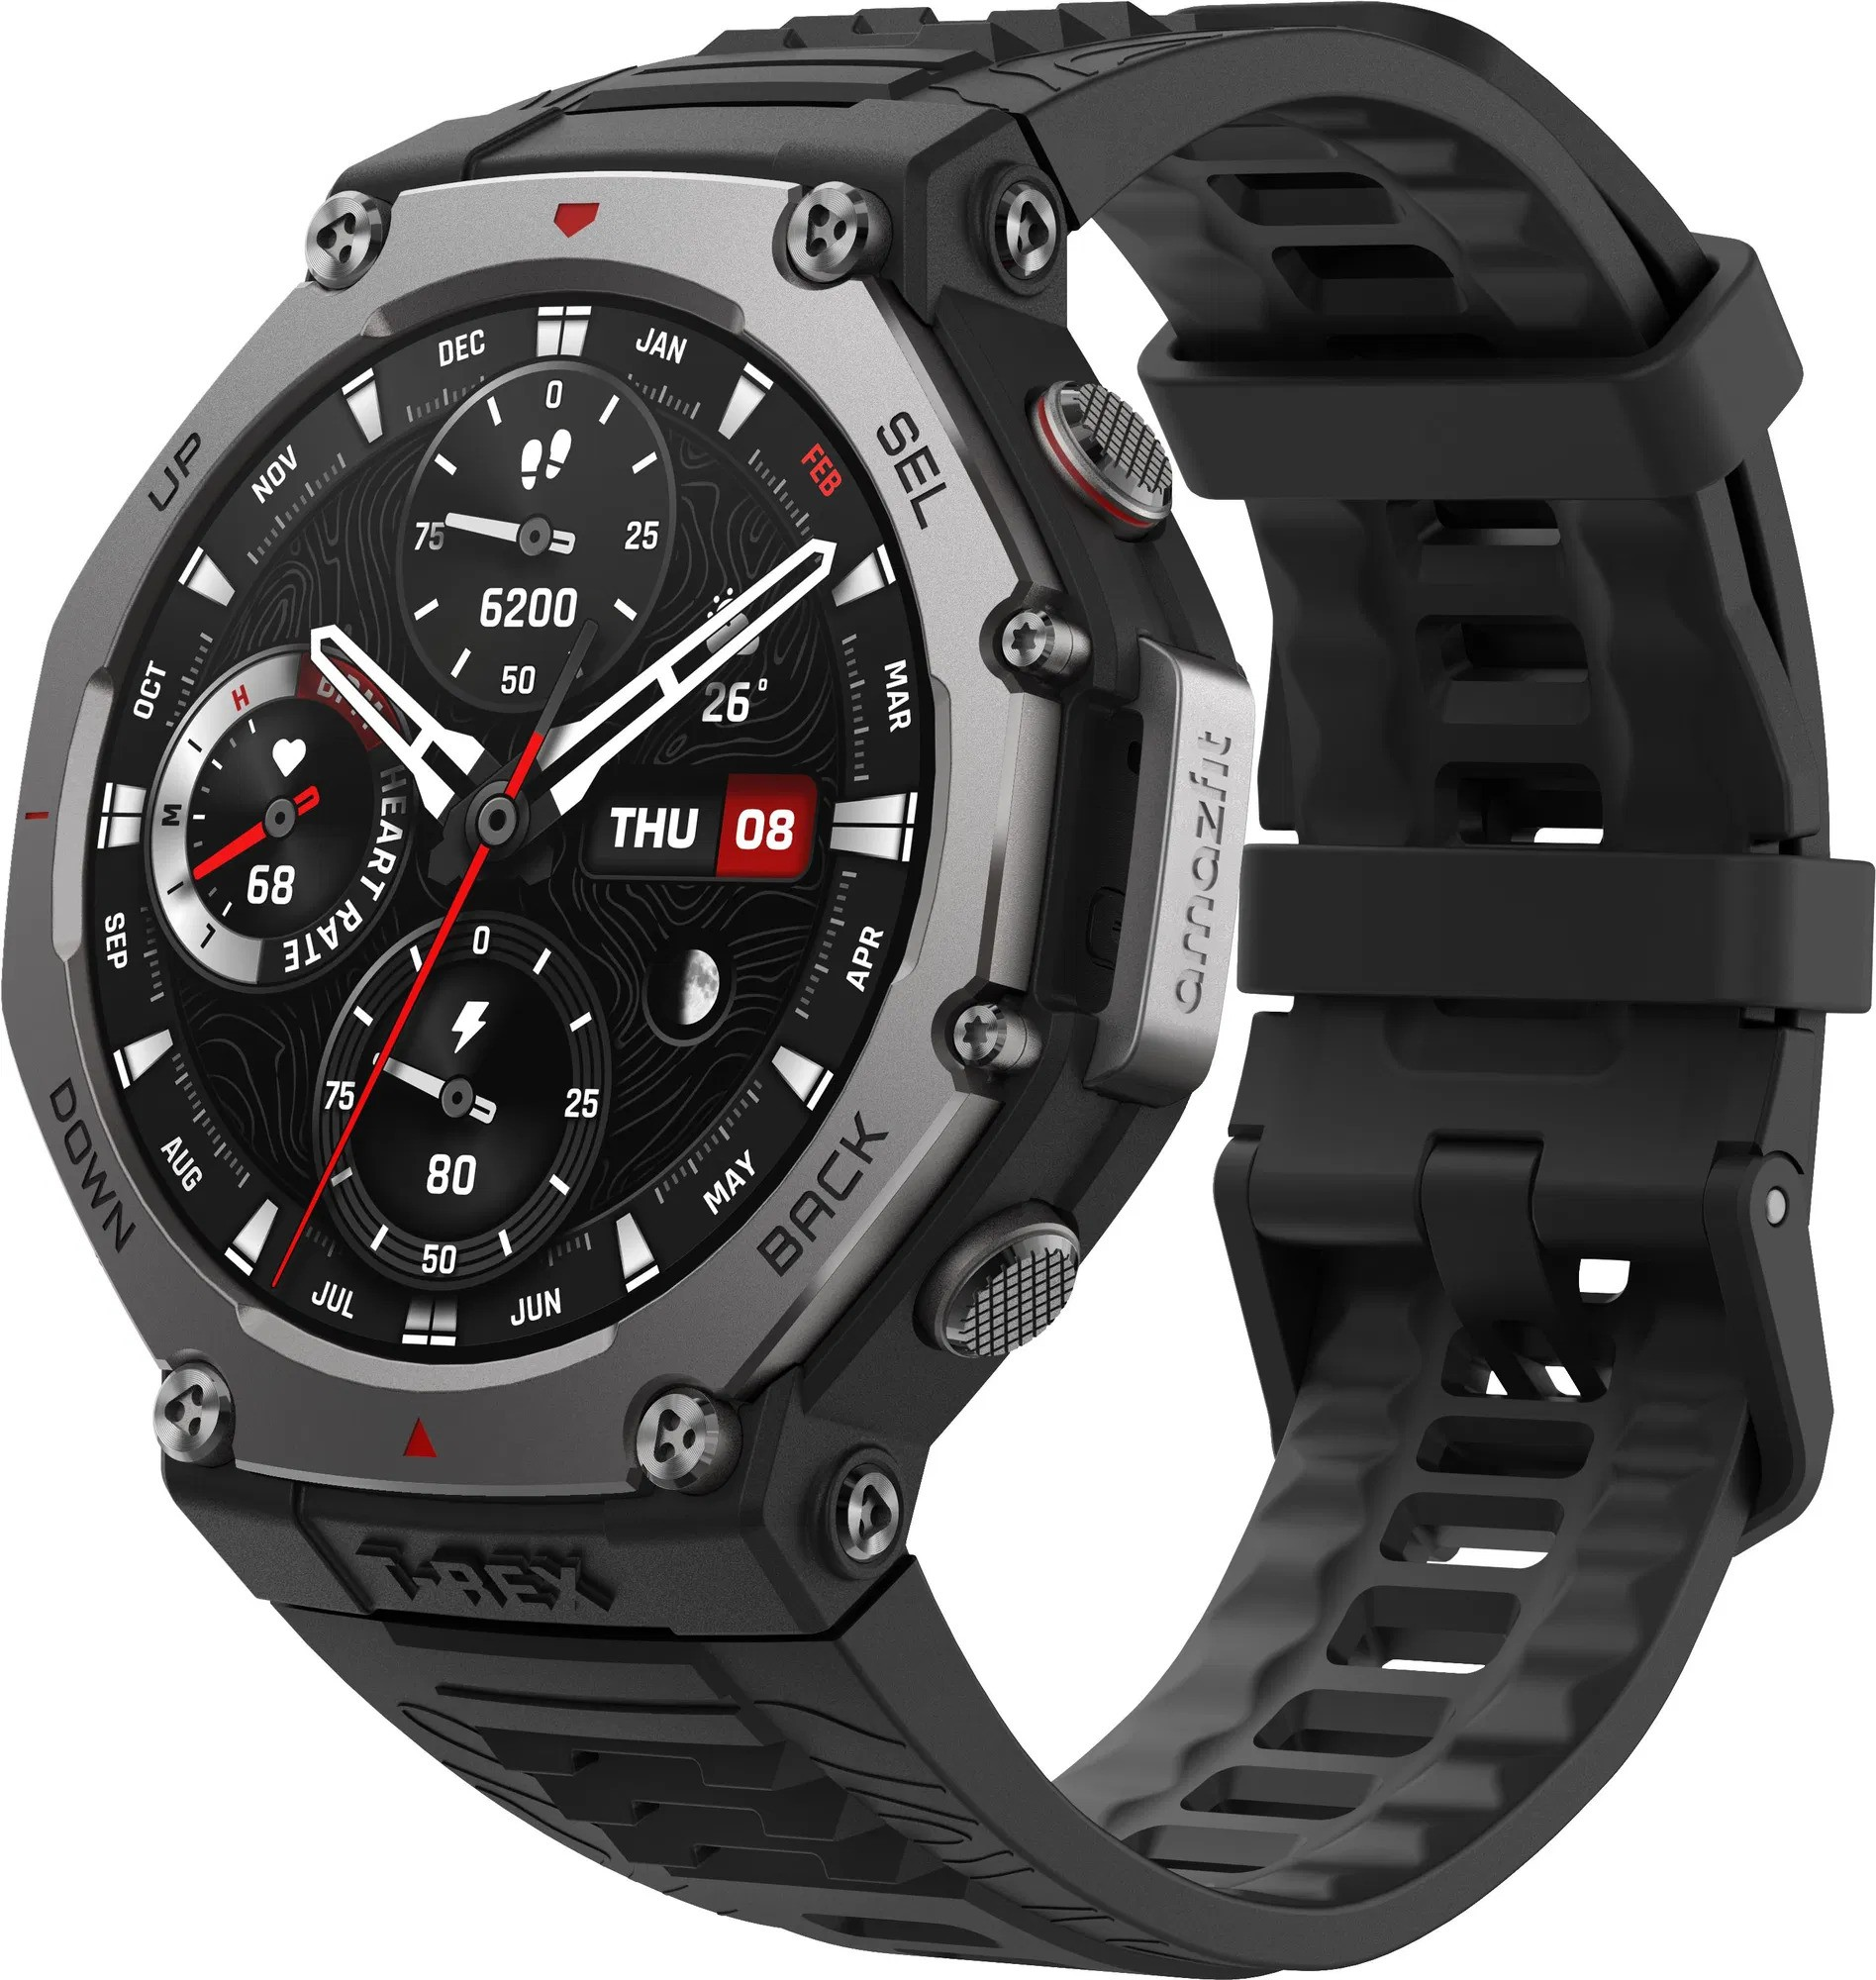
\includegraphics[width=0.5\linewidth]{img/trex3.jpg}
    \caption{Ukážka inteligentných hodiniek s~operačným systémom Zepp OS~\cite{amazfit-trex3-image}}
    \label{fig:trex3-pic}
\end{figure}


\subsubsection{Zepp OS}

Zepp OS~\cite{Zepp} je operačný systém pre inteligentné
hodinky a~nositeľné zariadenia zameraný na správu
zdravia. Na vyššej vrstve umožňuje vývojárom vytvárať
aplikácie (Mini Programy) a~ciferníky hodiniek
prostredníctvom poskytovaného \Gls{api}.

\subsubsection{Kľúčové vlastnosti Zepp OS}

Zepp~OS prináša viacero pokročilých funkcií, ktoré rozširujú možnosti
inteligentných hodiniek. Jednou z~nich je \textbf{Zepp~Flow}~\cite{zepp-flow}
-- prirodzené hlasové rozhranie, ktoré umožňuje používateľom ovládať
zariadenia prostredníctvom bežnej reči bez potreby špecifických príkazov
alebo dotykov. Zepp~Flow je postavený na pokročilých modeloch umelej
inteligencie, čo zaručuje plynulú a~intuitívnu interakciu.

Operačný systém ďalej poskytuje \textbf{podporu pre Mini~Programy
a~ciferníky hodiniek}. Vďaka jednoduchému frameworku môžu vývojári
vytvárať a~implementovať vlastné mini aplikácie a~prispôsobené ciferníky,
čím sa rozširuje funkčnosť a~personalizácia zariadení.

Verzia Zepp~OS~4 prináša aj \textbf{rozšírené jazykové a~hlasové
schopnosti}~\cite{zepp-voice}. V~čase citovania zdroja v~roku~2025
boli podporované hlasové odpovede v~angličtine a~nemčine, pričom
ďalšie jazyky -- francúzština, taliančina, španielčina, japončina,
kórejčina a~portugalčina -- boli ohlásené ako pripravované. Toto
vylepšenie zabezpečuje personalizovaný zážitok pre používateľov
s~rôznymi jazykovými preferenciami.

\subsection{Senzory}

Inteligentné hodinky sú vybavené rôznymi senzormi~\cite{sensors-article}
v~závislosti od cenovej kategórie a~zamerania. Základné modely
zvyčajne disponujú akcelerometrom na sledovanie pohybu.
Prémiové zariadenia, ako hodinky Amazfit T-Rex 3 použité
v~tejto práci, prinášajú pokročilé technológie vrátane
oxymetrov na meranie hladiny kyslíka v~krvi či senzorov
na analýzu telesného a zdravotného stavu.

\subsubsection{Akcelerometer}

Akcelerometer~\cite{sensors-article} meria zrýchlenie
zariadenia v~troch osiach -- X, Y a~Z. Funguje na princípe
mikroelektromechanických systémov (\Gls{mems}),
kde malé pohyblivé štruktúry vnútri senzora
reagujú na zmenu polohy a~sily pôsobiacej na
hodinky.

V~praxi~\cite{sensors-article} umožňuje sledovať počet
krokov, prejdenú vzdialenosť či spálené kalórie. Využíva
sa aj na rozpoznávanie gest, ako je otočenie zápästia na
zapnutie displeja. Spoločne s~gyroskopom pomáha
presnejšie analyzovať pohyb a~orientáciu zariadenia.

\subsubsection{Gyroskop}
Gyroskop~\cite{sensors-article} meria uhlovú rýchlosť
a~orientáciu zariadenia v~troch osiach -- X, Y a~Z.
Rovnako ako akcelerometer je založený na technológii \Gls{mems}.
Na rozdiel od akcelerometra, ktorý sleduje lineárny
pohyb, gyroskop sa zameriava na rotačné pohyby.

V~praxi vylepšuje sledovanie pohybu
pri športe \cite{sensors-article} -- napríklad pri plávaní alebo bicyklovaní
dokáže rozlíšiť špecifické vzorce otáčania ruky.
Spoločne s~akcelerometrom poskytuje detailnejšie údaje
o~pohybe, čo je užitočné pri určovaní typu aktivity.

\subsubsection{Monitor srdcovej frekvencie}

Senzor srdcového tepu~\cite{sensors-article} meria
frekvenciu tepu pomocou optickej technológie známej ako
fotopletizmografia (PPG). Využíva LED svetlá, ktoré
prenikajú do kože a~snímajú zmeny v~prietoku krvi.
Je kľúčový pre sledovanie kondície, monitorovanie stresu
či kvality spánku.

\subsubsection{GPS}

\Gls{gps}~\cite{sensors-article} v~inteligentných
hodinkách prijíma signály zo satelitov na určenie presnej
polohy používateľa. Funguje nezávisle od telefónu
a~umožňuje sledovať trasu, vzdialenosť či rýchlosť
pri aktivitách ako beh, cyklistika alebo turistika.
V~kombinácii s~akcelerometrom a~gyroskopom zvyšuje
presnosť navigácie.